% !TEX root = main.tex
\section{実験}

\subsection{実験内容}
本研究では,各アルゴリズム(PN,MPN,GS-MPN)の性能を比較し,追従精度や滑らかさ,安定性を評価する.
また,実環境でのシステム全体の動作を検証する.

\subsubsection{実験条件}
簡易的似作成した2輪移動ロボットを使用した.
実験は屋内環境で行った.以下に示すように人を直線運動時と曲線運動時とを追従させ,追従性能,
およびロボットのなめらかさを検証する.
\begin{itemize}
    \item \textbf{条件1}: 人(ターゲット)が直線に動く
    \item \textbf{条件2}: 人(ターゲット)が曲線に動く
\end{itemize}

また,以下に各設定パラメータを示す.

\begin{itemize}
    \item \textbf{比例ゲインv}: 5000
    \item \textbf{比例ゲインomega}: 50.0
    \item \textbf{最大微分ゲイン}: 0.1
    \item \textbf{動的微分ゲイン調整パラメータ}: 0.1
    \item \textbf{比例航法定数(N)}: 0.1
    \item \textbf{サンプリング間隔}: 0.1[s]
\end{itemize}

図\ref{fig:robo}に実験の様子とロボットを示す.

\begin{figure}[H]
    \centering
    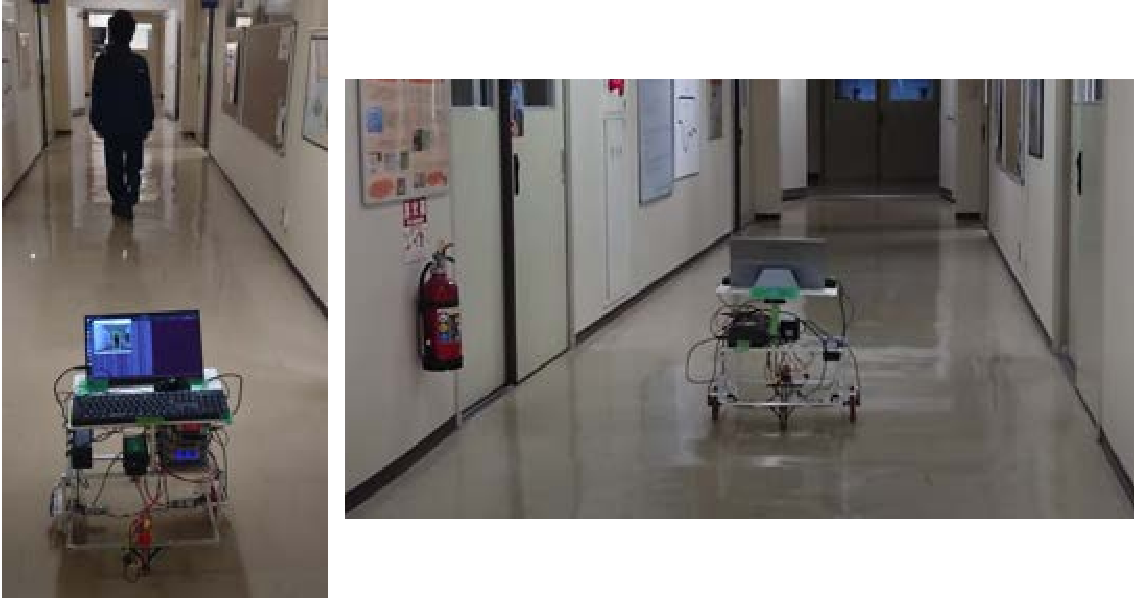
\includegraphics[width=0.8\textwidth]{figure/robo.pdf}
    \caption{実験の様子}
    \label{fig:robo}
\end{figure}

\subsubsection{実験の手順}
各アルゴリズムについて,以下の手順で実験を行った.
\begin{enumerate}
    \item ロボットの前(1[m])に追従物(人)を配置し,カメラの中心に来ていることを確認して実験を始める.
    \item 開始後,人が条件1,2に則り10[m]移動.
    \item エンコーダーデータやカメラデータを記録.
    \item 記録したcsvファイルを解析.
    \item これを3つのアルゴリズム,2つの条件で実験を行う.
\end{enumerate}

\subsection{実験結果及び考察}
本実験では,各アルゴリズム(PN,MPN,GS-MPN)の性能を比較するために,以下の指標を計測した.
\begin{itemize}
    \item \textbf{MeanOffset (px)}: ターゲット中心からの平均オフセット
    \item \textbf{StdOffset (px)}: オフセットの標準偏差
    \item \textbf{MeanAccel (mm/s²)}: 平均加速度
    \item \textbf{StdAccel (mm/s²)}: 加速度の標準偏差
\end{itemize}

表\ref{tab:experiment_results}に,各アルゴリズムの実験結果を示す.
また,図\ref{fig:offset_results}にMeanOffsetとStdOffset,図\ref{fig:accel_results}にMeanAccelとStdAccelのグラフを示す.

\begin{table}[H]
    \centering
    \caption{各アルゴリズムの実験結果}
    \label{tab:experiment_results}
    \resizebox{\textwidth}{!}{%
        \begin{tabular}{|l|c|c|c|c|}
            \hline
            \textbf{Experiment} & \textbf{MeanOffset (px)} & \textbf{StdOffset (px)} & \textbf{MeanAccel (mm/s²)} & \textbf{StdAccel (mm/s²)} \\ \hline
            PN\_data1           & 41.86                    & 54.03                   & 29.08                      & 29109.58                  \\ \hline
            PN\_data2           & 59.89                    & 64.74                   & 128.51                     & 27609.34                  \\ \hline
            MPN\_data1          & 102.42                   & 57.05                   & 202.61                     & 27873.37                  \\ \hline
            MPN\_data2          & 36.15                    & 51.27                   & 55.08                      & 11523.68                  \\ \hline
            GS-MPN\_data1       & 66.29                    & 69.30                   & 101.00                     & 11177.16                  \\ \hline
            GS-MPN\_data2       & 48.94                    & 69.98                   & 50.11                      & 21241.42                  \\ \hline
        \end{tabular}%
    }
\end{table}


\begin{figure}[H]
    \centering
    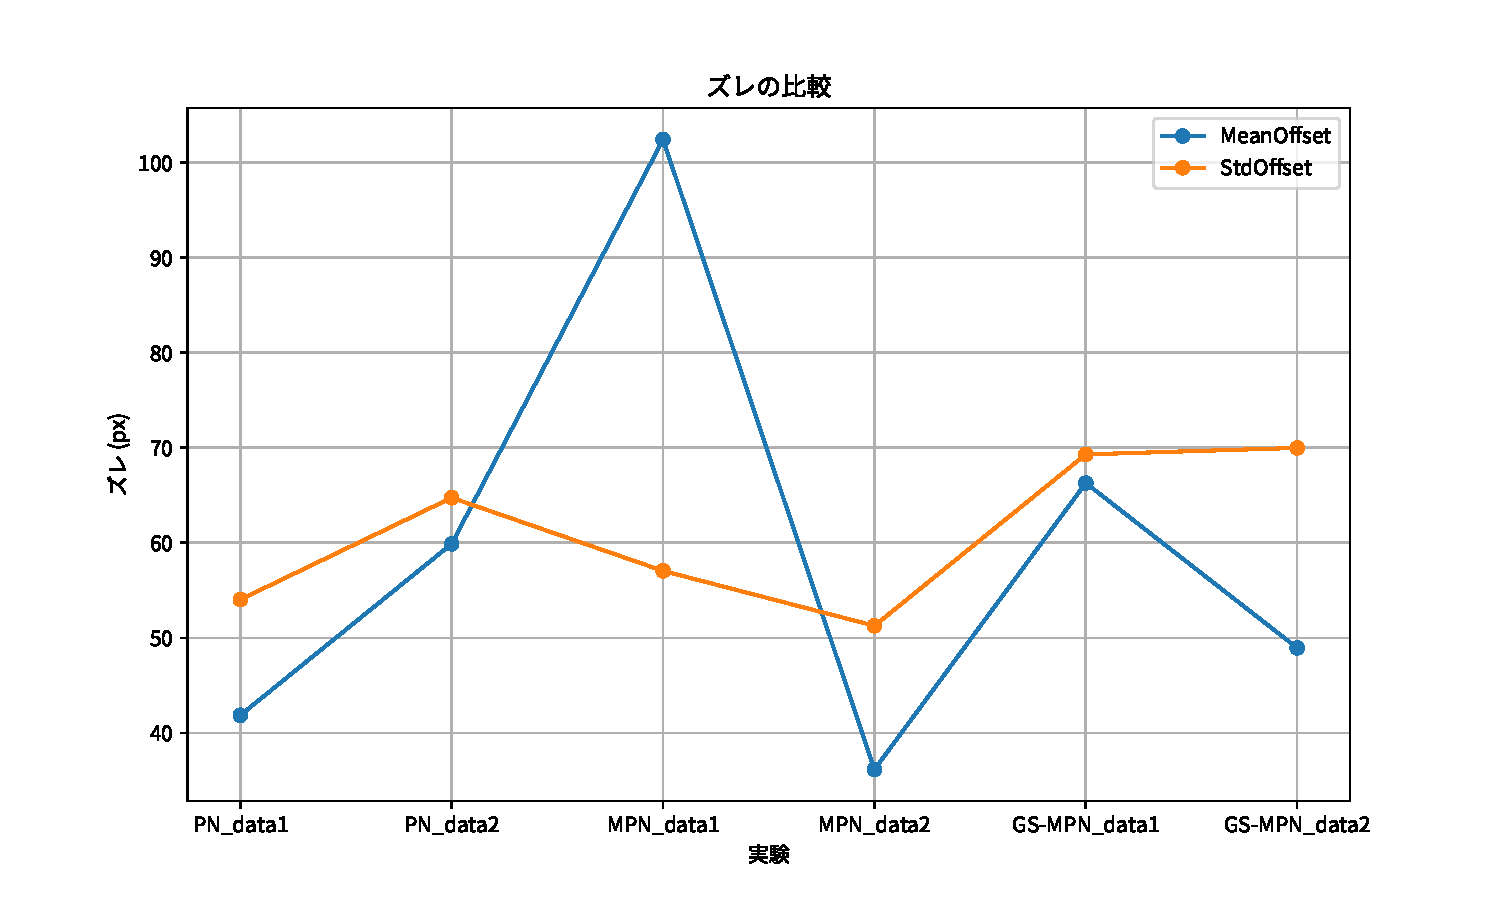
\includegraphics[width=1\textwidth]{figure/Offset.pdf}
    \caption{MeanOffsetおよびStdOffsetの比較}
    \label{fig:offset_results}
\end{figure}

\begin{figure}[H]
    \centering
    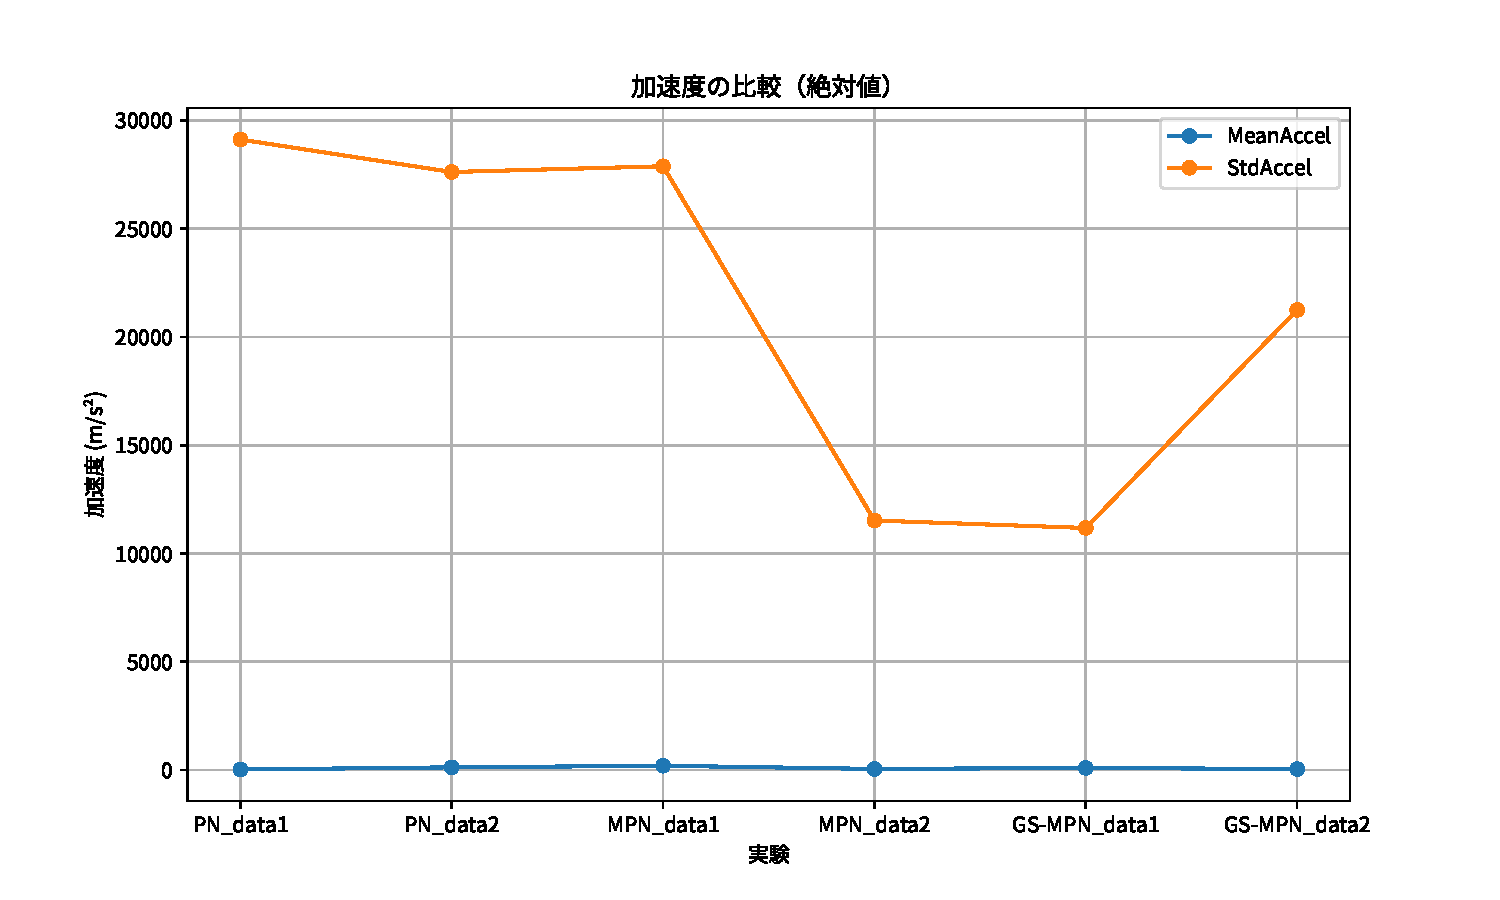
\includegraphics[width=1\textwidth]{figure/Accel.pdf}
    \caption{MeanAccelおよびStdAccelの比較}
    \label{fig:accel_results}
\end{figure}

\subsubsection{追従性能(MeanOffsetとStdOffset)}
追従性能を評価するために,MeanOffset(画面中心からのズレの平均値)とStdOffset(ズレの標準偏差)を用いた.
この指標は,目標物が画面内で中心付近にどれだけ正確に保持されているかを示す.
表\ref{tab:offset_results}に各アルゴリズムの結果を示す.

\begin{table}[H]
    \centering
    \caption{追従性能の評価結果}
    \label{tab:offset_results}
    \begin{tabular}{|l|c|c|}
        \hline
        \textbf{アルゴリズム} & \textbf{MeanOffset (px)} & \textbf{StdOffset (px)} \\ \hline
        PN\_data1             & 41.86                    & 54.03                   \\ \hline
        PN\_data2             & 59.89                    & 64.74                   \\ \hline
        MPN\_data1            & 102.42                   & 57.05                   \\ \hline
        MPN\_data2            & 36.15                    & 51.27                   \\ \hline
        GS-MPN\_data1         & 66.29                    & 69.30                   \\ \hline
        GS-MPN\_data2         & 48.94                    & 69.98                   \\ \hline
    \end{tabular}
\end{table}

PNは直線追従時に最も良好なMeanOffsetを示したが,曲線追従ではズレが大きくなり安定性が低下した.
一方で,MPNは逆の結果で曲線追従時にズレが減少し,直線追従時にズレが大きくなった.
特にGS-MPNは,直線追従時と曲線追従時の両方でバランスの良い結果を示している.

\subsubsection{スムーズさ(MeanAccelとStdAccel)}
スムーズさの指標として,MeanAccel(加速度の平均値)とStdAccel(加速度のばらつき)を用いた.
これらはロボットの動作の安定性と滑らかさを評価する.表\ref{tab:accel_results}に結果を示す.

\begin{table}[H]
    \centering
    \caption{スムーズさの評価結果}
    \label{tab:accel_results}
    \begin{tabular}{|l|c|c|}
        \hline
        \textbf{アルゴリズム} & \textbf{MeanAccel (mm/s²)} & \textbf{StdAccel (mm/s²)} \\ \hline
        PN\_data1             & 29.08                      & 29109.58                  \\ \hline
        PN\_data2             & 128.51                     & 27609.34                  \\ \hline
        MPN\_data1            & 202.61                     & 27873.37                  \\ \hline
        MPN\_data2            & 55.08                      & 11523.68                  \\ \hline
        GS-MPN\_data1         & 101.00                     & 11177.16                  \\ \hline
        GS-MPN\_data2         & 50.11                      & 21241.42                  \\ \hline
    \end{tabular}
\end{table}

PNは加速度のばらつき(StdAccel)が非常に大きく,急加速が多発する結果となった.
MPNでは曲線追従時に加速度が抑えられ,StdAccelが減少した.
特に GS-MPN は,直線追従時と曲線追従時の両方でバランスの良い結果を示している.

\subsubsection{視野内追従率(InFrameRate)}
視野内追従率(InFrameRate)は,目標物がカメラの視野内に保持されている割合を示す.
すべてのアルゴリズムで視野内追従率は100\%を記録し,目標物が常に視野内に維持されていることが確認された.

\subsubsection{総合評価}
本実験では,各アルゴリズム(PN,MPN,GS-MPN)を対象に追従性能,スムーズさ,および視野内追従率を評価した.

まず,PN(Proportional Navigation)は直線追従性能において最も良好な結果を示した.MeanOffsetが最小値を記録し,
目標物を中心付近に保持する能力が高いことが確認された.
一方で,StdOffsetが増加する傾向があり,特に曲線追従時にはズレが顕著になることが課題として挙げられる.
また,加速度のばらつき(StdAccel)が他のアルゴリズムに比べて極めて大きく,急激な動作が多発する結果となった.
このことから,PNは直線的な動作には適しているものの,動的環境や急な方向転換を必要とする状況では不安定性が課題となる.

次に,MPN(Modified Proportional Navigation)は,PNと比較して曲線追従性能と動作の滑らかさが大幅に改善された.
特にStdAccelの減少により,加速度のばらつきが抑制され,急激な加速や減速が少ない安定した動作が確認された.
さらに,MPN\_data2では,MeanOffsetとStdOffsetの値が他の条件よりも小さく,曲線追従における追従精度と安定性のバランスが良好であることが示されている.
しかしながら,直線追従時にはMeanAccelが最大値を記録しており,急加速が発生する傾向が見られた.
これは,微分項の影響が過大である可能性を示唆しており,直進時の制御パラメータの最適化が求められる.

最後に,GS-MPN(Gain-Scheduled Modified Proportional Navigation)は,全体的に最もバランスの取れた性能を示した.
動的微分ゲインを導入することで,急加速を抑制しながら安定した追従動作を実現していることが,MeanAccelおよびStdAccelの大幅な低下から確認された.
さらに,曲線追従においてもズレが抑制され,MPNよりも安定性が向上している.
一方で,MeanOffsetがPNと比較してやや大きい値を示しており,直線追従精度のさらなる向上が課題として挙げられる.
これには,動的微分ゲインの調整や,追加の制御項を導入することが効果的であると考えられる.

本実験の結果から,GS-MPNは滑らかな追従動作を必要とするシナリオにおいて最も有効であることが示唆された.
直線および曲線追従の両方において安定性が向上し,加速度のばらつきが最小化されることで,ロボットの動作がより自然で滑らかになることが確認された.
一方で,追従精度を向上させるための追加的な制御パラメータの調整や,動的環境における性能検証が今後の研究課題として残されている.
